\documentclass[tikz]{standalone}
\begin{document}

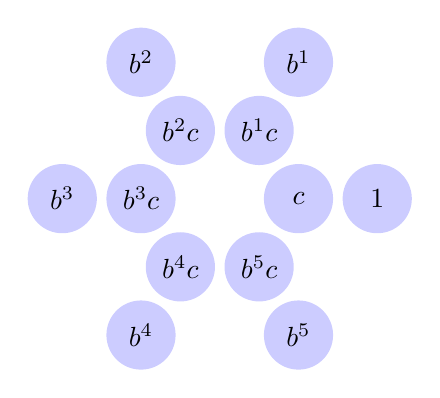
\begin{tikzpicture}
% Radius of regular polygons
\newdimen\Radi
\Radi=1cm
    % Indicate the boundary of the regular polygons
%    \draw [thin,black!20] circle (\Radi) ;
%    \fill[black!20] circle (2pt);
%    \draw (0:\Radi) \foreach \x in {120,240} {
%            -- (\x:\Radi)
%        } -- cycle (90:\Radi) node[above] {$n=3$} ;
%    \draw[xshift=2.5\Radi] (0:\Radi) \foreach \x in {90,180,...,359} {
%            -- (\x:\Radi)
%        } -- cycle (90:\Radi) node[above] {$n=4$} ;
%    \draw[xshift=5.0\Radi] (0:\Radi) \foreach \x in {72,144,...,359} {
%            -- (\x:\Radi)
%        } -- cycle (90:\Radi) node[above] {$n=5$} ;
        \foreach \x in {1,...,5} { %60,120,...,359} {
                \node[circle,minimum size=2.5em,fill=blue!20] at ({\Radi*cos(60*\x)},{\Radi*sin(60*\x)}) {\(b^{\x}c\)};
                \node[circle,minimum size=2.5em,fill=blue!20] at ({2*\Radi*cos(60*\x)},{2*\Radi*sin(60*\x)}) {\(b^{\x}\)};
		}
        \node[circle,minimum size=2.5em,fill=blue!20] at ({\Radi},{0}) {\(c\)};
        \node[circle,minimum size=2.5em,fill=blue!20] at ({2*\Radi},{0}) {\(1\)};        
            
%        % 360/7 = 51.4286 For PGF v < 1.18 we have to round to the nearest
%        % integer. Newer version support fractional angle values.
%        % For a more accurate result use the sequence
%        % {51, 103, 154, 206, 257, 309}
%        %
%        \draw[xshift=2.5\Radi] (0:\Radi) \foreach \x in {51.4286,102.8571,...,359} {
%                -- (\x:\Radi)
%            }-- cycle (90:\Radi) node[above] {$n=7$} ;
%        \draw[xshift=5.0\Radi] (0:\Radi) \foreach \x in {45,90,...,359} {
%                -- (\x:\Radi)
%            } -- cycle (90:\Radi) node[above] {$n=8$} ;
%    \draw[yshift=-6.0\Radi] (0:\Radi) \foreach \x in {10,20,...,359} {
%            -- (\x:\Radi)
%        } -- cycle (90:\Radi) node[above] {$n=36$} ;
\end{tikzpicture}
\end{document}
